\documentclass[bachelor, och, labwork]{shiza}
% параметр - тип обучения - одно из значений:
%    spec     - специальность
%    bachelor - бакалавриат (по умолчанию)
%    master   - магистратура
% параметр - форма обучения - одно из значений:
%    och   - очное (по умолчанию)
%    zaoch - заочное
% параметр - тип работы - одно из значений:
%    referat    - реферат
%    coursework - курсовая работа (по умолчанию)
%    diploma    - дипломная работа
%    pract      - отчет по практике
% параметр - включение шрифта
%    times    - включение шрифта Times New Roman (если установлен)
%               по умолчанию выключен
\usepackage{subfigure}
\usepackage{tikz,pgfplots}
\pgfplotsset{compat=1.5}
\usepackage{float}

%\usepackage{titlesec}
\setcounter{secnumdepth}{4}
%\titleformat{\paragraph}
%{\normalfont\normalsize}{\theparagraph}{1em}{}
%\titlespacing*{\paragraph}
%{35.5pt}{3.25ex plus 1ex minus .2ex}{1.5ex plus .2ex}

\titleformat{\paragraph}[block]
{\hspace{1.25cm}\normalfont}
{\theparagraph}{1ex}{}
\titlespacing{\paragraph}
{0cm}{2ex plus 1ex minus .2ex}{.4ex plus.2ex}

% --------------------------------------------------------------------------%


\usepackage[T2A]{fontenc}
\usepackage[utf8]{inputenc}
\usepackage{graphicx}
\graphicspath{ {./images/} }
\usepackage{tempora}

\usepackage[sort,compress]{cite}
\usepackage{amsmath}
\usepackage{amssymb}
\usepackage{amsthm}
\usepackage{fancyvrb}
\usepackage{listings}
\usepackage{listingsutf8}
\usepackage{longtable}
\usepackage{array}
\usepackage[english,russian]{babel}

\usepackage[colorlinks=false]{hyperref}
\usepackage{url}

\usepackage{underscore}
\usepackage{setspace}
\usepackage{indentfirst} 
\usepackage{mathtools}
\usepackage{amsfonts}
\usepackage{enumitem}
\usepackage{tikz}


\newcommand{\eqdef}{\stackrel {\rm def}{=}}
\newcommand{\specialcell}[2][c]{%
\begin{tabular}[#1]{@{}c@{}}#2\end{tabular}}

\renewcommand\theFancyVerbLine{\small\arabic{FancyVerbLine}}

\newtheorem{lem}{Лемма}

\begin{document}

% Кафедра (в родительном падеже)
\chair{теоретических основ компьютерной безопасности и криптографии}

% Тема работы
\title{Отношение эквивалентности и отношение порядка}

% Курс
\course{3}

% Группа
\group{331}

% Факультет (в родительном падеже) (по умолчанию "факультета КНиИТ")
\department{факультета КНиИТ}

% Специальность/направление код - наименование
%\napravlenie{09.03.04 "--- Программная инженерия}
%\napravlenie{010500 "--- Математическое обеспечение и администрирование информационных систем}
%\napravlenie{230100 "--- Информатика и вычислительная техника}
%\napravlenie{231000 "--- Программная инженерия}
\napravlenie{10.05.01 "--- Компьютерная безопасность}

% Для студентки. Для работы студента следующая команда не нужна.
% \studenttitle{Студентки}

% Фамилия, имя, отчество в родительном падеже
\author{Токарева Никиты Сергеевича}

% Заведующий кафедрой
% \chtitle{} % степень, звание
% \chname{}

%Научный руководитель (для реферата преподаватель проверяющий работу)
\satitle{аспирант} %должность, степень, звание
\saname{В. Н. Кутин}

% Руководитель практики от организации (только для практики,
% для остальных типов работ не используется)
% \patitle{к.ф.-м.н.}
% \paname{С.~В.~Миронов}

% Семестр (только для практики, для остальных
% типов работ не используется)
%\term{8}

% Наименование практики (только для практики, для остальных
% типов работ не используется)
%\practtype{преддипломная}

% Продолжительность практики (количество недель) (только для практики,
% для остальных типов работ не используется)
%\duration{4}

% Даты начала и окончания практики (только для практики, для остальных
% типов работ не используется)
%\practStart{30.04.2019}
%\practFinish{27.05.2019}

% Год выполнения отчета
\date{2022}

\maketitle

% Включение нумерации рисунков, формул и таблиц по разделам
% (по умолчанию - нумерация сквозная)
% (допускается оба вида нумерации)
% \secNumbering

%-------------------------------------------------------------------------------------------

\section{Постановка задачи}

    \textbf{Цель работы} - изучение основных свойств бинарных отношений и операций замыкания бинарных отношений. 

    Порядок выполнения работы:
    \begin{enumerate}
        \item Разобрать определения отношения эквивалентности, фактор-множества. Разработать алгоритмы построения
        эквивалентного замыкания бинарного отношения и системы представителей фактор-множества.
        \item Разобрать определения отношения порядка и диаграммы Хассе. Разработать алгоритмы вычисления минимальных
        (максимальных) и наименьших (наибольших) элементов  и построения диаграммы Хассе.
        \item Разобрать определения контекста и концепта. Разработать алгоритм вычисления решетки концептов.
    \end{enumerate}

\section{Теоретические сведения по рассмотренным темам с их обоснованием}

    \subsection{Определение отношения эквивалентности и фактор-множества}

        Бинарное отношение $\varepsilon$ на множестве $A$ называется отношением эквивалентности (или просто эквивалентностью), если оно рефлексивно, симметрично и транзитивно.

        Для любого подмножества $X \subset A$ множество $\rho(X) = \{b \in B: (x, b) \in \rho \text{ для некоторого } x \in X\}$ называется образом множества $X$ относительно отношения $\rho$.

        Образ одноэлементного множества $X = \{a\}$ относительно отношения $\rho$ обозначается символом $\rho(a)$ и называется также образом элемента $a$ или \textbf{срезом} отношения $\rho$ через элемент $a$. 

        Срезы $\varepsilon(a)$ называются классами эквивалентности по отношению $\varepsilon$ и сокращенно обозначаются символом $[a]$. Множество всех таких классов эквивалентности $\{[a]: a \in A\}$ называется фактор-множеством множества $A$ по эквивалентности $\varepsilon$ и обозначается символом $A/\varepsilon$.

        \textbf{Лемма 1.} О замыканиях бинарных отношений.

        На множестве $P(A^2)$ всех бинарных отношений между элементами множества $A$ следующие отображения являются
        операторами замыканий:

        \begin{enumerate}
            \item $f_r(\rho) = \rho \cup \triangle_A$ - наименьшее рефлексивное бинарное отношение, содержащее отношение
            $\rho \subset A^2$,
            \item $f_s(\rho) = \rho \cup \rho^{-1}$ - наименьшее симметричное бинарное отношение, содержащее отношение
            $\rho \subset A^2$,
            \item $f_t(\rho) = \bigcup^\infty_{n=1} \rho^{n}$ - наименьшее транзитивное бинарное отношение, содержащее
            отношение $\rho \subset A^2$,
            \item $f_{eq}(\rho) = f_t f_s f_r(\rho)$ - наименьшее отношение эквивалентности, на содержащее отношение
            $\rho \subset A^2$.
        \end{enumerate}        

    \subsection{Определение отношения порядка}

        Бинарное отношение $\omega$ на множестве $A$ называется отношением порядка (или просто порядком), если оно
        рефлексивно, антисимметрично и транзитивно.

        Множество $A$ с заданным на нем отношением порядка $\leq$ называется упорядоченным множеством и обозначается $A
        = (A, \leq)$ или просто $(A, \leq)$.

        Элемент $a$ упорядоченного множества $(A, \leq)$ называется:
        \begin{enumerate}
            \item минимальным, если $(\forall x \in A) \text{ } x \leq a \implies x = a$,
            \item максимальным, если $(\forall x \in A) \text{ } a \leq x \implies x = a$,
            \item наименьшим, если $(\forall x \in A) \text{ } a \leq x$,
            \item наибольшим, если $(\forall x \in A) \text{ } x \leq a$.
        \end{enumerate}

    \subsection{Определение диаграммы Хассе}

        Упорядоченное множество $A = (A, \leq)$ наглядно представляется диаграммой Хассе, которая представляет элементы множества $A$ точками плоскости и пары $a <\cdot \text{ } b$ представляет линиями, идущими вверх от элемента $a$ к элементу $b$.

        Алгоритм построения диаграммы Хассе конечного упорядоченного множества $A = (A, \leq)$.

        \begin{enumerate}
            \item В упорядоченном множестве $A = (A, \leq)$ найти множество $A_1$ всех минимальных элементов и расположить их в один горизонтальный ряд (это первый уровень диаграммы).
            \item В упорядоченном множестве $A \setminus A_1$, найти множество $A_2$ всех минимальных элементов и
            расположить их в один горизонтальный ряд над первым уровнем (это второй уровень диаграммы). Соединить
            отрезками элементы этого ряда с покрываемыми ими элементами предыдущего ряда.
            \item В упорядоченном множестве $A \setminus (A_1 \cup A_2)$ найти множество $A_3$ всех минимальных
            элементов и расположить их в один горизонтальный ряд над вторым уровнем (это третий уровень диаграммы).
            Соединить отрезками элементы этого ряда с покрываемыми ими элементами предыдущих рядов.
            \item Процесс продолжается до тех пор, пока не выберутся все элементы множества $A$.
        \end{enumerate}

    \subsection{Определение контекста и концепта}

        Контекстом называется алгебраическая система $K = (G, M, \rho)$, состоящая из множества объектов $G$, множества атрибутов $M$ и бинарного отношения $\rho \subset G \times M$, показывающего $(g, m) \in \rho$, что объект $g$ имеет атрибут $m$.

        Упорядоченная пара $(X, Y)$ замкнутых множеств $X \in Z_{f_G}, Y \in Z_{f_M}$, удовлетворяющих условиям $\varphi(X) = Y$, $\psi(Y) = X$, называется концептом контекста $K = (G, M, \rho)$. При этом компонента $X$ называется объемом и компонента $Y$ - содержанием концепта $(X, Y)$.

        Множество всех концептов $C(K)$ так упорядочивается отношением \\ $(X, Y) \leq (X_1, Y_1) \Leftrightarrow X \subset X_1$ (или равносильно $Y_1 \subset Y$), что $(C(K), \leq)$ является полной решеткой, которая изоморфна решетке замкнутых подмножеств множества $G$.

        Алгоритм вычисления системы замыканий на множестве $G$:
        \begin{enumerate}
            \item Рассматриваем множество $G \in Z_{f_G}$.
            \item Последовательно перебираем все элементы $m \in M$ и вычисляем для них $\psi(\{m\}) = \rho^{-1}(m)$.
            \item Вычисляем все новые пересечения множества $\psi(\{m\})$ с ранее полученными множествами и добавляем новые множества к $Z_{f_G}$. Аналогично вычисляется система замыканий на множестве $M$.
        \end{enumerate}

\section{Результаты работы}
    \subsection{Описание алгоритма построения эквивалентного замыкания бинарного отношения и системы представителей
    фактор-множества}

        \underline{Алгоритм 1 - Построение эквивалентного замыкания}\\
            \textit{Вход}: Матрица бинарного отношения $A = (a_{ij})$ размерности $n \times n$.\\
            \textit{Выход}: Матрица бинарного отношения $A' = (a'_{ij})$ с построенным на нем эквивалентным
            замыканием.\\
            \underline{Шаг 1.} Построить рефлексивное замыкание на бинарном отношении с матрицей $A = (a_{ij})$.
            Полученную матрицу бинарного отношения обозначить как $A_1 = (a_{ij})$.\\
            \underline{Шаг 2.} Построить симметричное замыкание на бинарном отношении с матрицей $A_1 = (a_{ij})$.
            Полученную матрицу бинарного отношения обозначить как $A_2 = (a_{ij})$.\\
            \underline{Шаг 3.} Построить транзитивное замыкание на бинарном отношении с матрицей $A_2 = (a_{ij})$.
            Полученную матрицу бинарного отношения обозначить как $A' = (a'_{ij})$.\\
            \underline{Шаг 4.} Согласно пункту 4 леммы 1 о замыканиях бинарных отношений, построенное замыкание на
            данном бинарном отношении, определяемым матрицей, является эквивалентным. Далее вернуть полученную матрицу
            $A' = (a'_{ij})$.\\
            
            Трудоемкость алгоритма $O(n^3)$.\\

        \underline{Алгоритм 2 - Построение системы представителей фактор-множества}\\
            \textit{Вход}: Матрица бинарного отношения $A = (a_{ij})$ размерности $n \times n$.\\
            \textit{Выход}: Система представителей $T$ фактор-множества $A/\varepsilon$ бинарного отношения на множестве $A$.\\
            \underline{Шаг 1.} Получить фактор-множество $A/\varepsilon$ бинарного отношения для множества $A$. Для
            этого нужно получить классы эквивалентности $\varepsilon(a)$, которые являются срезами по элементам
            множества $A$. Срезом по каждому элементу $a \in A$ является совокупность таких элементов множества $A$, значения которых в строке матрицы, определяющей связи между элементом $a$ и другими элементами множества $A$, равны единице. Для этого проверим элементы $a_{ij}$ матрицы $A$, и если $a_{ij} = 1$, где $0 \leq i, j \leq n - 1$, то добавить значение $j$ в список, определяющий срез по элементу $i$. В результате полученная совокупность всех таких срезов, являющихся классами эквивалентности $\{[a]: a \in A\}$, будет определять фактор-множество $A/\varepsilon$ бинарного отношения $A$.\\ 
            \underline{Шаг 2.} Отсортировать фактор-множество по возрастанию количества элементов в классах эквивалентности.\\
            \underline{Шаг 3.} Проходясь по каждому элементу $a$ каждого класса эквивалентности $[a]$ проверять: если элемент $a$ класса эквивалентности не находится в системе представителей - добавить элемент в систему представителей как представителя класса эквивалентности $[a]$, иначе - пропустить элемент.\\
            \underline{Шаг 4.} Вернуть полученную систему представителей.\\
            
            Трудоемкость алгоритма $O(n^2)$.\\

    \subsection{Описание  алгоритмов  вычисления  минимальных  (максимальных)  и  наименьших (наибольших) элементов и
    построения диаграммы Хассе}

        \underline{Алгоритм 3 - Вычисление минимального элемента множества}\\
            \textit{Вход}: Матрица бинарного отношения $A = (a_{ij})$ размерности $n \times n$.\\
            \textit{Выход}: Список минимальных элементов $L$ упорядоченного множества $(A, \leq)$.\\
            \underline{Шаг 1.} Получить срезы по элементам с помощью способа, описанного в алгоритме 2: проверить
            элементы $a_{ij}$ матрицы $A$, и если $a_{ij} = 1$, где $0 \leq i, j \leq n - 1$, то добавить значение $j$ в
            список, определяющий срез по элементу $i$. В результате получить список срезов $S = \{s_i = [a]: a \in A\}$,
            размер которого будет $n$. \\
            \underline{Шаг 2.} Добавить в список минимальных элементов $L$ первый по счету элемент $a_0$ множества $A$,
            а в качестве максимальной возможной длины среза $max(|s|)$ указать длину среза $s_0$.\\
            \underline{Шаг 3.} Проверить элементы $s_i$ списка срезов $S$, где $1 \leq i, j \leq n - 1$: если $max(|s|)
            < |s_i|$, то $max(|s|)$ сделать равным длине среза $|s_i|$ по элементу $a_i$, а список минимальных элементов
            очистить и добавить в него элемент $a_i \in A$. Иначе, если $max(|s|) = |s_i|$, то добавить в список
            минимальных элементов $L$ элемент $a_i \in A$. \\
            \underline{Шаг 4.} Вернуть список минимальных элементов $L$ упорядоченного множества $(A, \leq)$.\\

            Трудоемкость алгоритма $O(n^2)$.\\

        \underline{Алгоритм 4 - Вычисление максимального элемента множества}\\
            \textit{Вход}: Матрица бинарного отношения $A = (a_{ij})$ размерности $n \times n$.\\
            \textit{Выход}: Список максимальных элементов $L$ упорядоченного множества $(A, \leq)$.\\
            \underline{Шаг 1.} Получить срезы по элементам с помощью способа, описанного в алгоритме 2: проверить
            элементы $a_{ij}$ матрицы $A$, и если $a_{ij} = 1$, где $0 \leq i, j \leq n - 1$, то добавить значение $j$ в
            список, определяющий срез по элементу $i$. В результате получить список срезов $S = \{s_i = [a]: a \in A\}$,
            размер которого будет $n$. \\
            \underline{Шаг 2.} Добавить в список максимальных элементов $L$ первый по счету элемент $a_0$ множества $A$,
            а в качестве минимальной возможной длины среза $min(|s|)$ указать длину среза $s_0$.\\
            \underline{Шаг 3.} Проверить элементы $s_i$ списка срезов $S$, где $1 \leq i, j \leq n - 1$: если $min(|s|)
            > |s_i|$, то $min(|s|)$ сделать равным длине среза $|s_i|$ по элементу $a_i$, а список максимальных
            элементов очистить и добавить в него элемент $a_i \in A$. Иначе, если $min(|s|) = |s_i|$, то добавить в
            список максимальных элементов $L$ элемент $a_i \in A$. \\
            \underline{Шаг 4.} Вернуть список максимальных элементов $L$ упорядоченного множества $(A, \leq)$.\\

            Трудоемкость алгоритма $O(n^2)$.\\

        \underline{Алгоритм 5 - Вычисление наименьшего элемента множества}\\
            \textit{Вход}: Матрица бинарного отношения $A = (a_{ij})$ размерности $n \times n$.\\
            \textit{Выход}: Наименьший элемент $a_{min}$ упорядоченного множества $(A, \leq)$ или ''Ничего''.\\
            \underline{Шаг 1.} Получить список $L$ минимальных элементов упорядоченного множества $(A, \leq)$ с помощью алгоритма 3. \\
            \underline{Шаг 2.} Если длина $L$ не равна $1$, вернуть ''Ничего'', иначе - вернуть единственный элемент $a_{min} = l \in L$, являющийся наименьшим элементом множества $A$.\\
                
            Трудоемкость алгоритма $O(n^2)$.\\

        \underline{Алгоритм 6 - Вычисление наибольшего элемента множества}\\
            \textit{Вход}: Матрица бинарного отношения $A = (a_{ij})$ размерности $n \times n$.\\
            \textit{Выход}: Наибольший элемент $a_{max}$ упорядоченного множества $(A, \leq)$ или ''Ничего''.\\
            \underline{Шаг 1.} Получить список $L$ максимальных элементов упорядоченного множества $(A, \leq)$ с помощью
            алгоритма 4. \\
            \underline{Шаг 2.} Если длина $L$ не равна $1$, вернуть ''Ничего'', иначе - вернуть единственный элемент
            $a_{max} = l \in L$, являющийся наибольшим элементом множества $A$.\\
                
            Трудоемкость алгоритма $O(n^2)$.\\

        \underline{Алгоритм 7 - Построение диаграммы Хассе}\\
            \textit{Вход}: Матрица бинарного отношения порядка $A = (a_{ij})$ размерности $n \times n$.\\
            \textit{Выход}: Список $H$ длиной $n$, характеризующий диаграмму Хассе: каждый элемент в списке представляет
            собой три значения: элемент $a \in A$, значение его уровня $l$ на диаграмме, список $V$ элементов множества
            $A$, находящихся на уровне $l + 1$ и связанных с элементом $a$. \\
            \underline{Шаг 1.} Определить копию матрицы $A = (a_{ij})$ как $A' = (a'_{ij})$ и копию множества $A$ как
            $A'$, а также список $L$, в котором будут храниться значения уровня $l$ для каждого элемента $a \in A$.
            Изначально присвоить всем элементам $l \in L$ уровень $1$. Также определить счетчик уровней $i = 1$.\\
            \underline{Шаг 2.} Получить список $L_{min}$ минимальных элементов множества $A$ с помощью алгоритма 3, отправив ему на вход матрицу бинарного отношения порядка $A = (a_{ij})$.\\
            \underline{Шаг 3.} Для каждого элемента $a$ в $L_{min}$ соответствующее ему значение списка $l \in L$
            сделать равным $i$. После чего удалить $a$ из множества $A'$ (и удалить строку матрицы $A' = (a'_{ij})$,
            которая соответствует элементу $a$). Затем увеличить значение $i$ на $1$.\\
            \underline{Шаг 4.} Если множество $A'$ не пустое, перейти на шаг $2$.\\
            \underline{Шаг 5.} Определить пустой список $V$. Проходясь по элементам списка $L$, где $0 \leq k \leq n -
            1$, определять для каждого значения $l_k$ пустой список $v_k$ связанных с элементом $a_k$ элементов
            множества $A$. Определяя такой список, далее проходить по элементам $a_{ij}$ матрицы $A$, где $0 \leq i, j
            \leq n - 1$: если значение $a_{ij} = 1$ и уровень $l_i \in L$ элемента $a_i \in A$ равен $l_k + 1$, то
            добавить элемент $a_i$ в список $v_k$. После этого отсортировать список $v_k$ и добавить его в $V$. \\
            \underline{Шаг 6.} Создать список $H$ и поместить в него в качестве элемента $h_i \in H$ тройку значений:
            $a_i \in A$, $l_i \in L$, $v_i \in V$, где $0 \leq i \leq n - 1$. После этого вернуть список $H$. \\

            Трудоемкость алгоритма $O(n^3)$.\\

    \subsection{Описание алгоритма построения решетки концептов}

        \underline{Алгоритм 8 - Построение системы замыканий}\\
            \textit{Вход}: Контекст $K = (G, M, \rho)$ с множеством объектов $G$, множеством атрибутов $M$ и отношением
            $\rho \subset G \times M$, заданного матрицей $A = (a_{ij})$ размерности $n \times k$ (где $n$ - количество
            объектов, $k$ - количество атрибутов). \\
            \textit{Выход}: Система замыканий $Z_{f_G}$ на множестве $G$.\\
            \underline{Шаг 1.} Определить список $Z_{f_G}$ и положить туда $G$. \\
            \underline{Шаг 2.} Получить срезы по атрибутам $m \in M$ с помощью способа, описанного в алгоритме 2:
            необходимо предварительно транспонировать матрицу $B = A^T = (a_{ij})^T = b_{ij}$, затем проверить элементы
            $b_{ij}$ матрицы $B$, и если $b_{ij} = 1$, где $0 \leq i \leq k - 1$ и $0 \leq j \leq n - 1$, то добавить
            значение объекта $g_j$ в список, определяющий срез по атрибуту $m_i$. В результате получить список срезов
            $S_G = \{s_i = [g]: g \in G\}$, размер которого будет $k$. \\
            \underline{Шаг 3.} Для каждого атрибута $m_i \in M$: определить список $T$, в который поместить $s_i \in
            S_G$. Далее для каждого замыкания $z_j$ из системы замыканий $Z_{f_G}$: получить пересечение множеств $s_i$
            и $z_j$ и обозначить его как $X = s_i \cap z_j$. Если $X$ не содержится в списке $T$: добавить $X$ в список
            $T$ (всё это осуществляется при $0 \leq i \leq k - 1$). Если $T \notin Z_{f_G}$, то положить $T$ в
            $Z_{f_G}$.\\
            \underline{Шаг 4.} Вернуть систему замыканий $Z_{f_G}$ на множестве $G$.\\

            Трудоемкость алгоритма $O(n^2 + n \cdot k)$.\\

        \underline{Алгоритм 9 - Построение решетки концептов}\\
            \textit{Вход}: Контекст $K = (G, M, \rho)$ с множеством объектов $G$, множеством атрибутов $M$ и отношением
            $\rho \subset G \times M$, заданного матрицей $A = (a_{ij})$ размерности $n \times k$ (где $n$ - количество
            объектов, $k$ - количество атрибутов). \\
            \textit{Выход}: Решетка концептов $(C(K), \leq)$. \\
            \underline{Шаг 1.} Построить систему замыканий $Z_{f_G}$ с помощью алгоритма 8, отправив ему на вход
            контекст $K = (G, M, \rho)$. \\
            \underline{Шаг 2.} Определить пустой список $(C(K), \leq)$.\\
            \underline{Шаг 3.} Построить список $P$ следующим образом: если $z_i = \emptyset$, то $P = M$, иначе -
            получить среды по объектам $G$ с помощью способа, описанного в алгоритме 2: проверить элементы $a_{rt}$
            матрицы $A$, и если $a_{rt} = 1$, где $0 \leq t \leq k - 1$ и $0 \leq r \leq n - 1$, то добавить значение
            $m_t$ в список, определяющий срез по объекту $g_r$. В результате получить список срезов $S_M = \{s_i = [m]:
            m \in M\}$, размер которого будет $n$. Определить пустой список $Y$. Далее для каждого объекта в замыкании
            $z_i$: добавить срез $s_i$, соответствующий конкретному объекту, в список $Y$. После этого осуществить
            пересечение всех срезов $s$, находящихся в списке $Y$, и поместить результат пересечения в список $P$. После
            построения $P$ добавить пару значений $z_i$ и $P$ в качестве элемента в список $(C(K), \leq)$.\\
            \underline{Шаг 4.} Проделать шаг 3 для всех элементов $Z_{f_G}$. После этого вернуть построенную решетку
            концептов $(C(K), \leq)$. \\

            Трудоемкость алгоритма $O(n^2 + n \cdot k + n^3)$.\\

    % \subsection{Коды программ, реализующей рассмотренные алгоритмы}

    %     \inputminted[fontsize=\small]{python}{code/lab-2.py}

    % \subsection{Результаты тестирования программ}
    %     \begin{figure}[H]
    %         \centering
    %         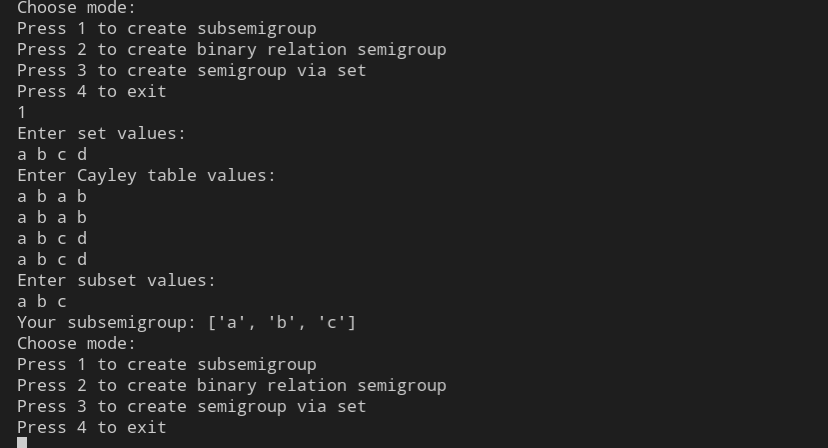
\includegraphics[width=0.8\textwidth]{pic/1.png}
    %         \caption{Тест алгоритма эквивалентного замыкания}
    %     \end{figure}

    %     \begin{figure}[H]
    %         \centering
    %         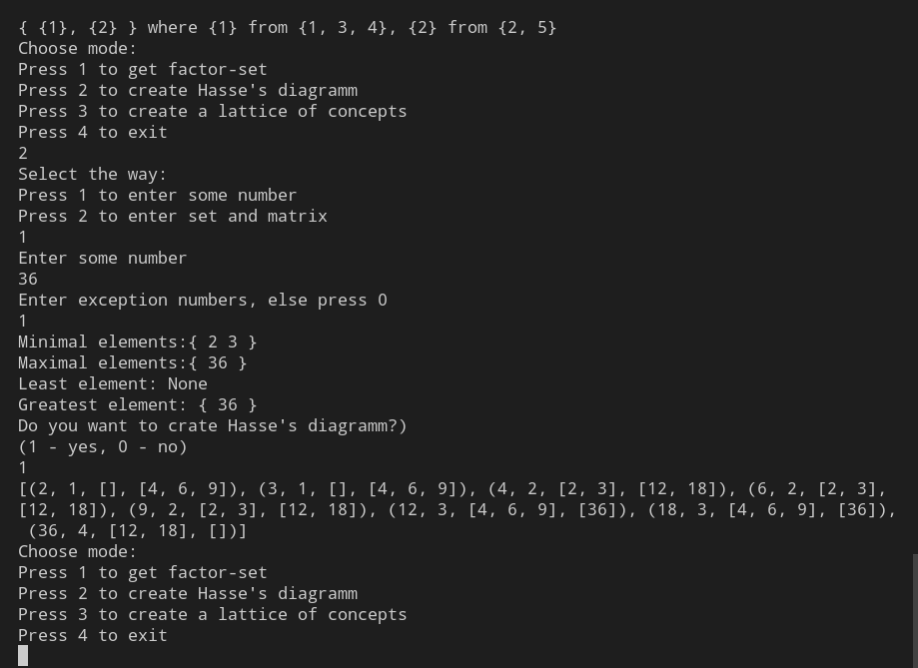
\includegraphics[width=1\textwidth]{pic/2.png}
    %         \caption{Тест алгоритма системы представителей}
    %     \end{figure}

    %     \begin{figure}[H]
    %         \centering
    %         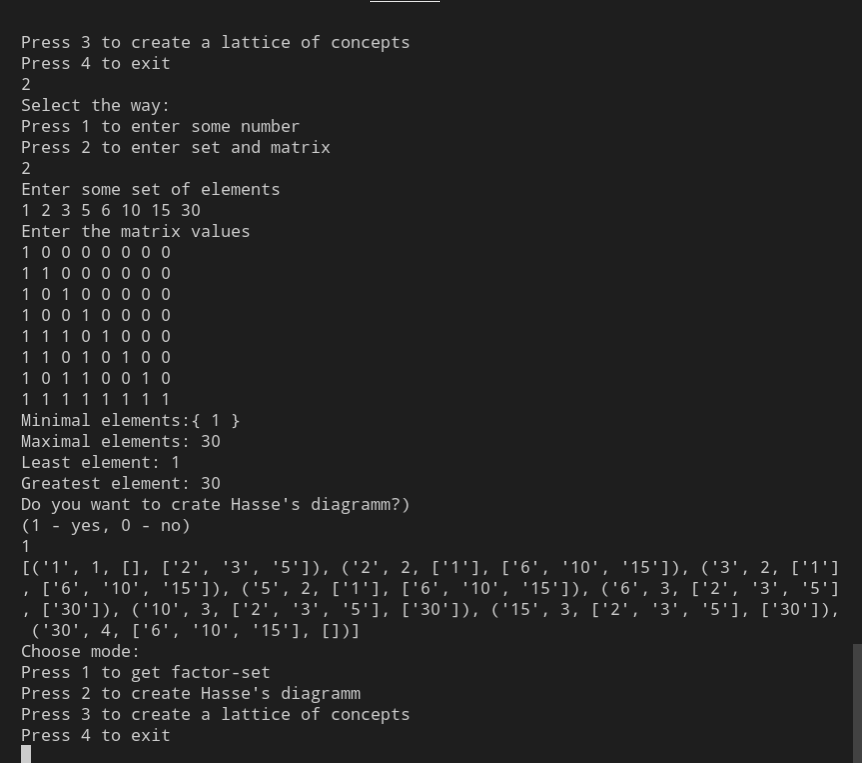
\includegraphics[width=0.8\textwidth]{pic/3.png}
    %         \caption{Тест нахождения минимальных (максимальных) и наименьших (наибольших) элементов множества}
    %     \end{figure}

    %     \begin{figure}[H]
    %         \centering
    %         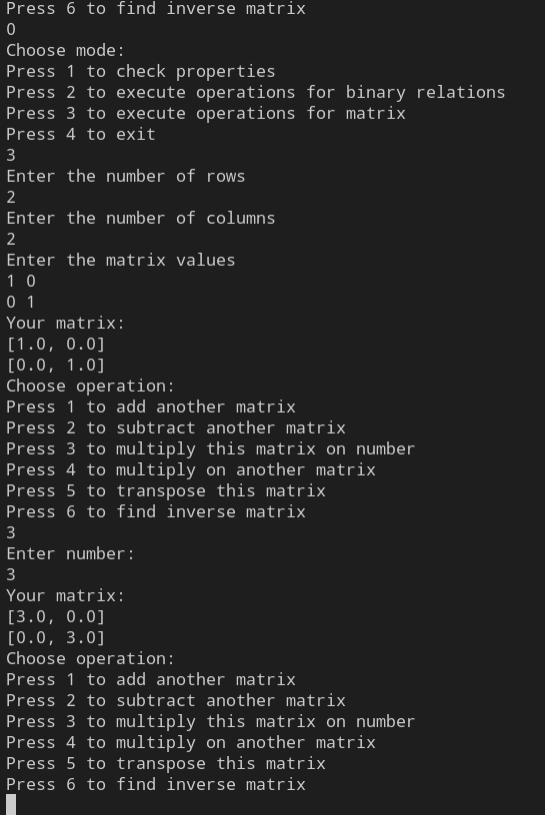
\includegraphics[width=1\textwidth]{pic/4.png}
    %         \caption{Тест алгоритма построения диаграммы Хассе}
    %     \end{figure}

    %     \begin{figure}[H]
    %         \centering
    %         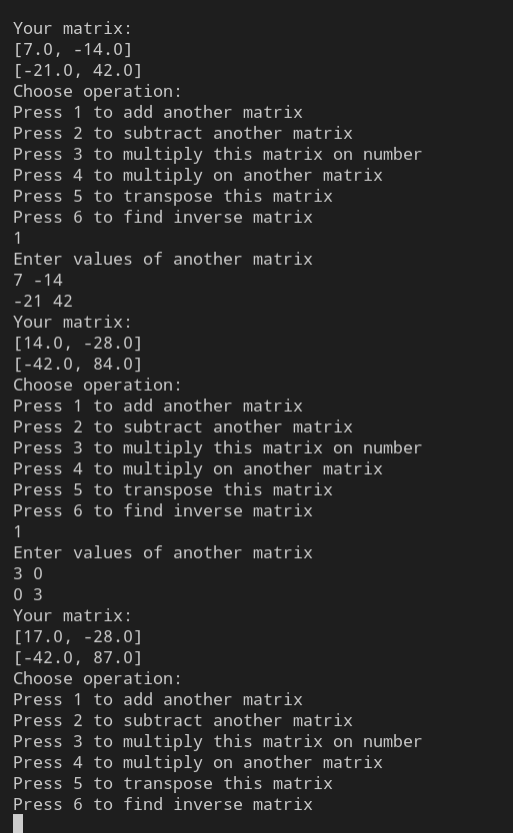
\includegraphics[width=1\textwidth]{pic/5.png}
    %         \caption{Тест алгоритма построения решетки концепта}
    %     \end{figure}

    \subsection{Оценки сложности рассмотренных алгоритмов}
    
        \textbf{Алгоритм эквивалентного замыкания.}\\
            В силу применения поочередно рефлексивного, симметричного и транзитивного замыкания, и с учетом
            результатов вычисления асимптотики для первой лабораторной работы, алгоритм эквивалентного замыкания имеет асимптотику $O(n^3)$.

        \textbf{Алгоритм системы представителей.}\\
            С учетом наличия одного вложенного цикла, алгоритм системы представителей имеет асимптотику $O(n^2)$.

        \textbf{Алгоритм нахождения минимальных (максимальных) и наименьших (наибольших) элементов множества.}\\
            С учетом наличия одного вложенного цикла, а также сходства между алгоритмами нахождения минимального и
            максимального элемента множества, а также взаимосвязи с алгоритмами нахождения наименьшего и наибольшего
            элемента множества, каждый из этих алгоритмов имеет асимптотику $O(n^2)$.

        \textbf{Алгоритм построения диаграммы Хассе.}\\
            С учетом наличия двух вложенных циклов, алгоритм построения диаграммы Хассе имеет асимптотику $O(n^3)$.
        
        \textbf{Алгоритм построения решетки концепта.}\\
            С учетом наличия двух пар вложенных циклов, где у одной пары 1-ый цикл осуществляется по множеству атрибутов
            (размерности $n$), а 2-ой - по множеству объектов (размерности $k$), а у другой пары два цикла по множеству
            размерности $n$, асимптотика составляет $O(n^2 + n \cdot k)$. Помимо этого, а также с учетом двух вложенных
            циклов, алгоритм построения диаграммы Хассе имеет асимптотику $O(n^2 + n \cdot k + n^3)$.

\conclusion

    В данной лабораторной работе были рассмотрены теоретические сведения об отношении эквивалентности, разобраны
    определения фактор-множества, отношения порядка и диаграммы Хассе, контекста и концепта. На их основе были
    составлены алгоритмы построения эквивалентного замыкания бинарного отношения и системы представителей
    фактор-множества, алгоритмы вычисления минимальных (максимальных) и наименьших (наибольших) элементов и построения
    диаграммы Хассе, а также алгоритмы построения решетки концептов. Была произведена оценка сложности созданных
    алгоритмов. Они послужили фундаментом для программной реализации, которая впоследствии успешно прошла тестирование,
    результаты которого были прикреплены к отчету вместе с листингом программы, написанной на языке Python с
    использованием библиотеки Numpy для работы с большими массивами данных.

\end{document}